\documentclass[ngerman, 12pt, pdftex]{scrartcl}[2006/07/30]

%encoding and input
\usepackage[ngerman]{babel} %spell correction
\usepackage[utf8]{inputenc} 
\usepackage[T1]{fontenc}

%bugfixes
\usepackage{fixltx2e} 

%Font Symbols and Colors
\usepackage{textcomp} %more symbols
\usepackage{xcolor}

%Math
\usepackage{amsmath}
\usepackage{mathtools} %extends amsmath

%Programming
\usepackage{listingsutf8} %in utf8
\lstset{language=Java,captionpos=b,tabsize=3,frame=,keywordstyle=\color{blue},commentstyle=\color{teal},stringstyle=\color{red},numbers=none,numberstyle=\tiny,numbersep=5pt,breaklines=false,showstringspaces=false,basicstyle=\footnotesize,emph={label},upquote=false} %Syntax highlighting

%Verbatim extension (with line numbers and tab-expansion)
\usepackage{moreverb} 

%Headers and Footer
\usepackage{fancyhdr}

%title
\title{Handbuch}
\author{Frank M\"{u}ller, Oliver Wisler, Luzius Bachmann, Fabio Sulser}
\subtitle{Swissdefcon-Team}

\begin{document}
%declare  Header
\pagestyle{fancy}
\fancyhf{} 
\fancyhead[L]{Handbuch} %left header
\fancyhead[C]{Swissdefcon-Team} %centered header
\fancyhead[R]{\thepage}  % right header
\renewcommand{\headrulewidth}{0.1pt} 	%upper separating line
%\fancyfoot[C]{\thepage} 				%centered footer, line number



%you might want to enable come features:
\maketitle
%\listoffigures 
%\listoftables


\newpage

\tableofcontents

\newpage

\section{Spiel starten}
\subsection{Kommandozeile}
\subsubsection{Server}
Der Server kann auf dem Standardport(9002) wie folgt gestartet werden:

\begin{lstlisting}
java -jar pfad.zum.jar server
\end{lstlisting}
Du kannst auch einen Port angeben, um den Server auf einem von dir definierten Port zu starten:
\begin{lstlisting}
java -jar pfad.zum.jar server PORT
\end{lstlisting}
           

\subsubsection{Client}
Der Client kann ohne Angaben wie folgt gestartet werden:
\begin{lstlisting}
java -jar pfad.zum.jar
\end{lstlisting}
Dabei fängt der Client automatisch an, verfügbare Server zu suchen. 
Es kann auch direkt versucht werden direkt zu einem Server zu verbinden, 
dabei ist eine Angabe des Servers sowie des zugehörigen Ports nötig.
Der Standardport des Servers ist 9002.
\begin{lstlisting}
java -jar pfad.zum.jar client IP:PORT 
\end{lstlisting}

\subsubsection{Server und Client}
Es kann gleichzeitig ein Client und ein Server gestartet werden.
Dabei wird der Server auf Standardport 9002 gestartet.
\begin{lstlisting}
java -jar pfad.zum.jar beides
\end{lstlisting}

\newpage

\subsection{Graphisch}
Starte den Client und melde dich folgendermassen an.

\begin{figure}[h]
\centering
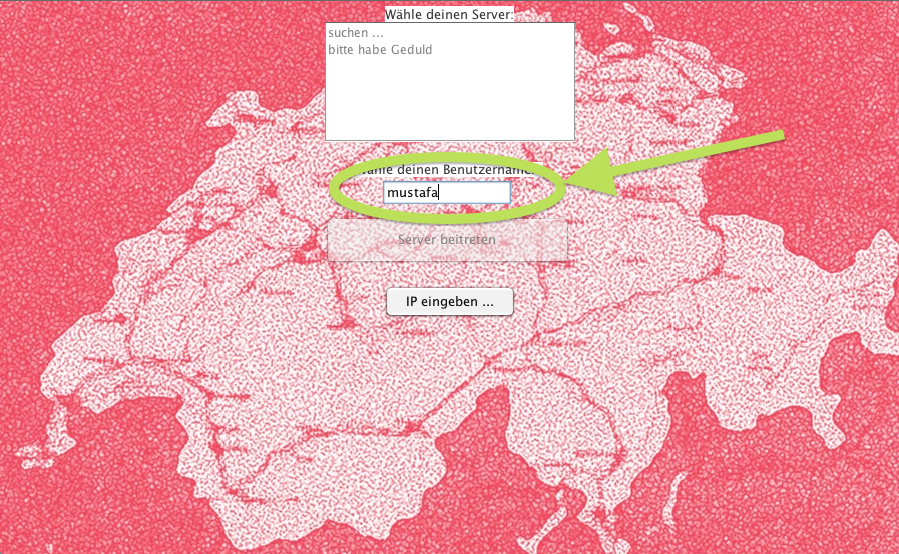
\includegraphics[scale=0.3]{starten/namen_eingeben.png}
\caption{Gib den Namen ein}
\end{figure}

Gib in dem markierten Feld deinen Namen ein. Standardm\"{a}ssig wird der Benutzername deines Computers verwendet.


\begin{figure}[h]
\centering
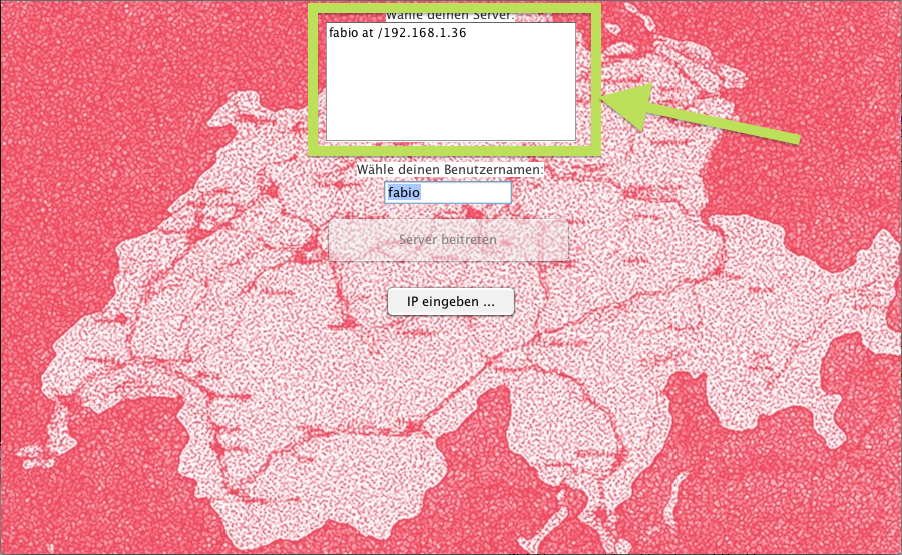
\includegraphics[scale=0.3]{starten/serverliste.png}
\caption{Liste der Server}
\end{figure}

In dem oben markierten Feld siehst du die Liste der aktiven Server.

\newpage 

\begin{figure}[h]
\centering
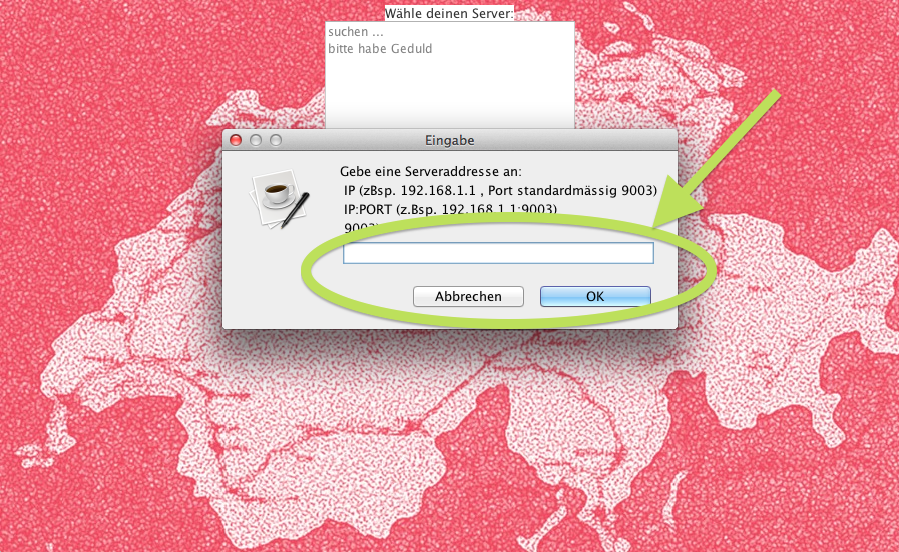
\includegraphics[scale=0.3]{starten/IP_manuell_eingeben.png}
\caption{Serveradresse eingeben}
\end{figure}

Gibt es einen Server, der nicht in der Liste angezeigt wird, so kannst du dessen Adresse auch von
Hand eingeben.


\begin{figure}[h]
\centering
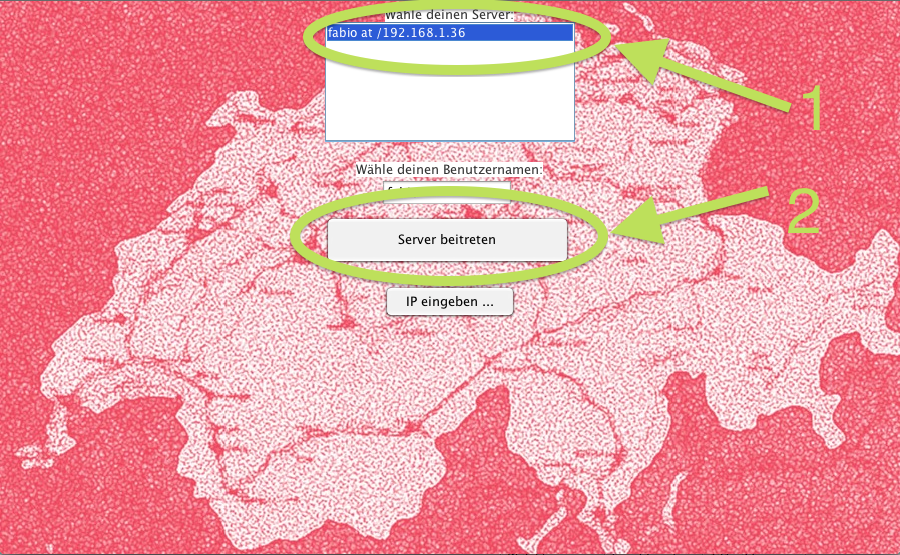
\includegraphics[scale=0.3]{starten/server_waehlen.png}
\caption{Server w\"{a}hlen}
\end{figure}

W\"{a}hle einen Server aus der ober beschriebenen Liste per Mausklick aus und gib deinen(1) und dr\"{u}cke dann auf "'Server betreten"'(2).

\newpage

\subsection{Verbindungsaufbau}
Hast du einen Server angegeben, so wird versucht die Verbindung zum Server herzustellen. Sobald du verbunden bist, erscheint die Lobby.
Falls keine Verbindung zum Server hergestellt werden kann,  wird die nachfolgende Meldung angezeigt. Du gehst wieder zurück zur Serverauswahl.
\begin{figure}[h]
\centering
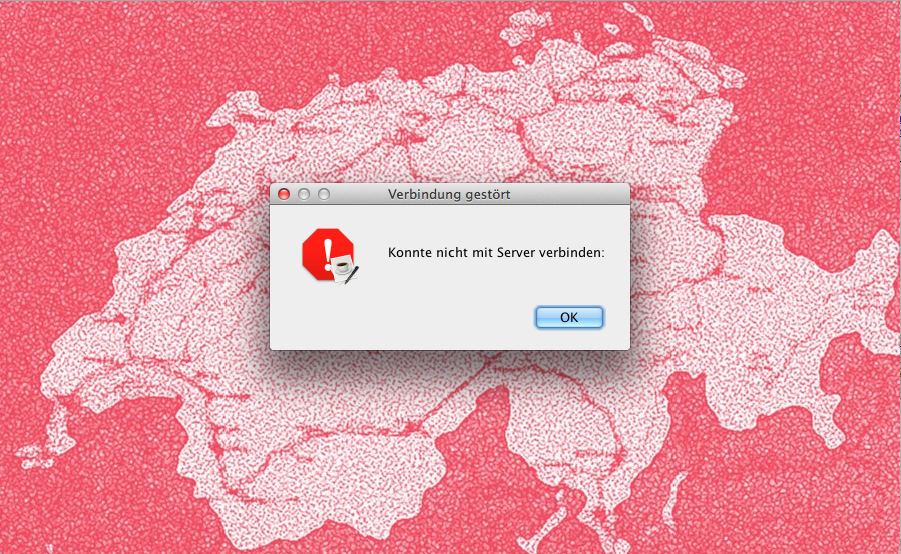
\includegraphics[scale=0.3]{starten/keine_serververbindung.png}
\caption{Fehler, keine Verbindung zum Server}
\end{figure}




\newpage

\section{Lobby}

Nun hast du es geschafft und bist in der Lobby.
\subsection{Chat}
Auf der rechten Seite siehst du das Chatfenster.
\begin{figure}[h]
\centering
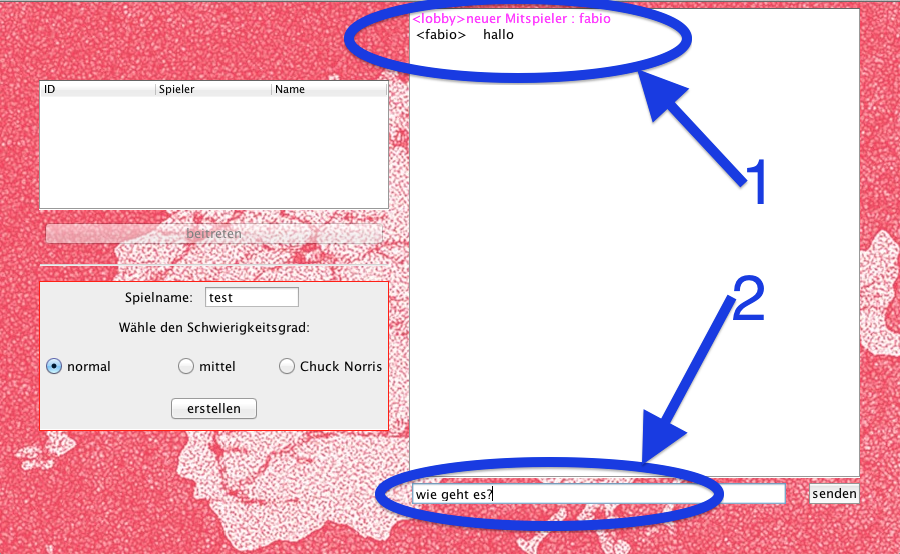
\includegraphics[scale=0.3]{lobby/chat.png}
\caption{Chat auf der Rechten Seite}
\end{figure}

In dem Chat kannst du nun Nachrichten von anderen Personen sehen, die sich auf dem selben Server wie du befinden. Zudem werden dir wichtige Informationen in dem Chatfenster angezeigt(1).
Unterhalb des Chat-Ausgabefensters siehst du das Eingabepanel, in dem du deine Nachricht eingeben kannst(2). Zum senden der Nachricht dr\"{u}cke entweder die Enter-Taste, oder dr\"{u}cke auf den senden-Button.
\subsubsection{Befehle}
Eine normale Chat-eingabe ist f\"{u}r alle Mitspieler sichtbar. \\
M\"{o}chtest du eine private Nachricht an eine Person senden, so gib den Befehl \lstinline{/MSG hans hallo} in das Eingabepanel ein, wobei "'hans"' der Name des anderen Spielers ist und "'hallo"' die Nachricht, die gesendet wird. \\
Um deinen Nicknamen zu wechseln, gib den Befehl \lstinline{/VNICK muster} in das Eingabepanel ein, wobei "'muster'" dein neuer Name ist.
Alle Eingaben welche ein führenden Backslash haben, werden direkt als Befehl an den Server geschickt. Damit ist es möglich von Hand Befehle an den Server zu schicken (zum Beispiel \lstinline{/VEXIT} beendet die Verbindung). Serverbefehle sind nicht case-sensitive.

\newpage

\subsection{Spiele}
M\"{o}chtest du ein neues Spiel erstellen oder betreten, so kannst du dies folgendermassen machen.

\begin{figure}[h]
\centering
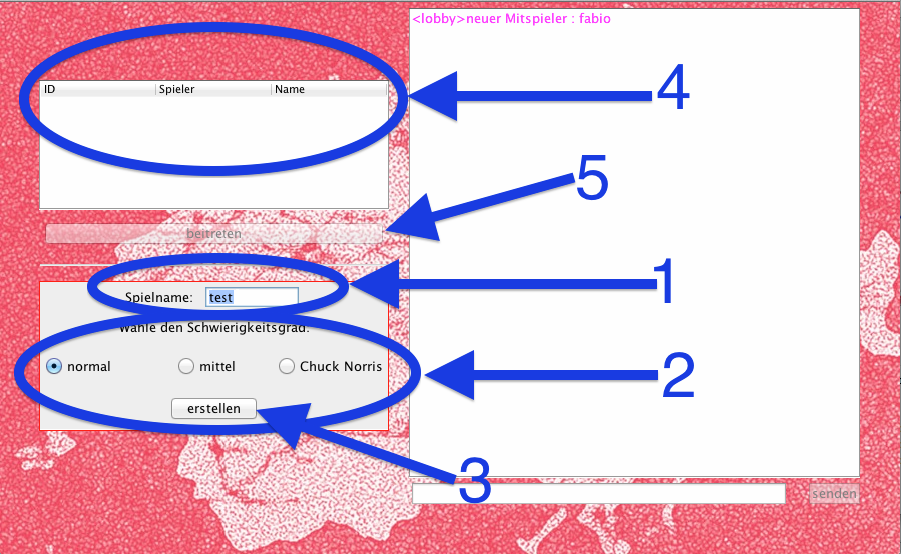
\includegraphics[scale=0.3]{lobby/spiel_erstellen.png}
\caption{Spiel erstellen oder beitreten}
\end{figure}

Um ein neues Spiel zu erstellen, so gib im Textfeld einen neuen Spielnamen ein(1).
Der Spielname muss mindestens aus 4 Buchstaben bestehen.
W\"{a}hle eine Schwierigkeitsstufe zwischen "'normal"', "'schnell"' oder "'Präsentation"' aus(2).
Um das erstellen des Spiels abzuschliessen dr\"{u}cke auf den Knopf erstellen.

Um einem bereits bestehenden Spiel beizutreten, so w\"{a}hle dieses per Mausklick in der Liste der Spiele (4) aus, und dr\"{u}cke dann auf den Knopf "'beitreten"'.

Danach gelangst du einen Schritt weiter. Hier siehst du einige Infos zum Spiel in dem du dich befindest.

\begin{figure}[h]
\centering
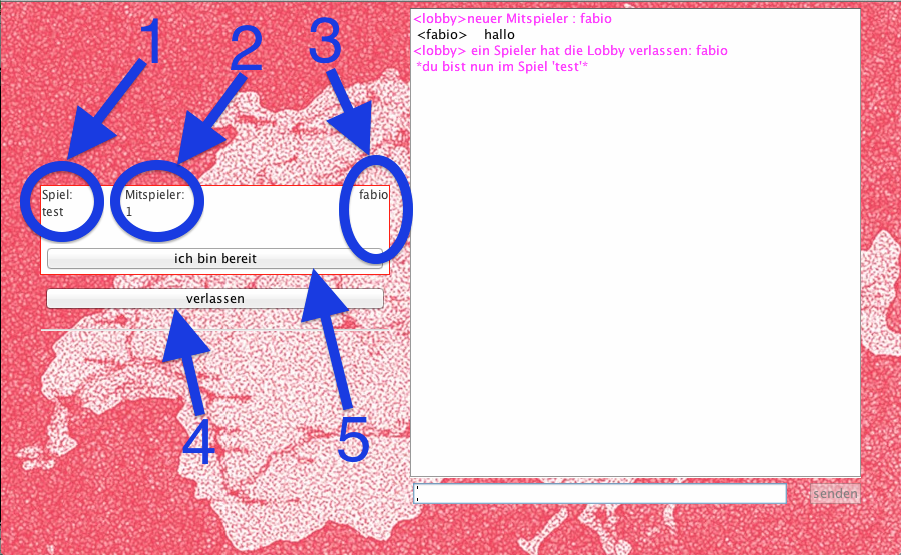
\includegraphics[scale=0.3]{lobby/spielinfos.png}
\caption{Spiel erstellen oder beitreten}
\end{figure}

 Ganz links steht der Name des Spiels(1), in der Mitte findest du die Anzahl der Mitspieler(2) und ganz rechts siehst du eine Liste mit den Namen deiner Mitspieler(3).
Um zur allgemeinen Lobby zur\"{u}ckzukehren dr\"{u}cke auf "'verlassen"'(4).
Wenn du bereit zum Spielen bist, dann dr\"{u}cke auf "'ich bin bereit"'(5). Sobald mehr als die Hälfte aller Mitspieler bereit ist, so beginnt das Spiel.

\newpage

\section{Spiel}
\subsection{Spielprinzip}
Im Jahre 2100 besteht die Schweiz aus 5 Grosskantonen. Jeder dieser Kantone hat den Anspruch die vollständige Macht in der Schweiz zu übernehmen.
Genauer heisst dies, dass du die Macht im Nationalrat übernehmen musst. Dies ist der Fall sobald alle anderen Kantone keine Bevölkerung mehr haben.
Du bist der Präsident eines dieser Kantone und hast das Ziel, deinen Kanton zum Herrscher über die Schweiz zu machen. 
Um deine Ziele zu erreichen stehen dir verschiedene Einheiten zur Verfügung, welche im Kapitel Einheiten erläutert werden.
Das Spiel ist rundenbasiert, das heisst, dass du jeweils eine Runde Zeit hast deine Züge zu machen und danach die Züge ausgeführt werden.

\subsection{Schwierigkeitsgrade}
\begin{itemize}
\item Normal mit grosser Population und wenig Geld
\item Schnell mit kleiner Population und viel Geld
\item Präsentation mit sehr kleiner Population und sehr viel Geld
\end{itemize}

\subsection{Spielfenster}
Hier eine Übersicht über das Spielfenster. Das Spiel wird im Vollbildmodus gestartet. Auf der rechten Seite ist der Chat, mit dem du mit allen Spielern im Spiel chatten kannst.
Unten rechts findest du den Zustand deines Kantons. Unten in der Mitte wird die verbleibende Zeit für diese Runde angezeigt. 
Direkt daneben ist das Panel mit welchem du Einheiten platzieren kannst, dazu wählst du einfach eine Einheit aus und platzierst sie auf deinem Feld (das blaue Feld).
Links findest du noch die Bedienbuttons zum Beenden des Spiel oder um deinen letzten Spielzug zu löschen.
\begin{figure}[h]
\centering
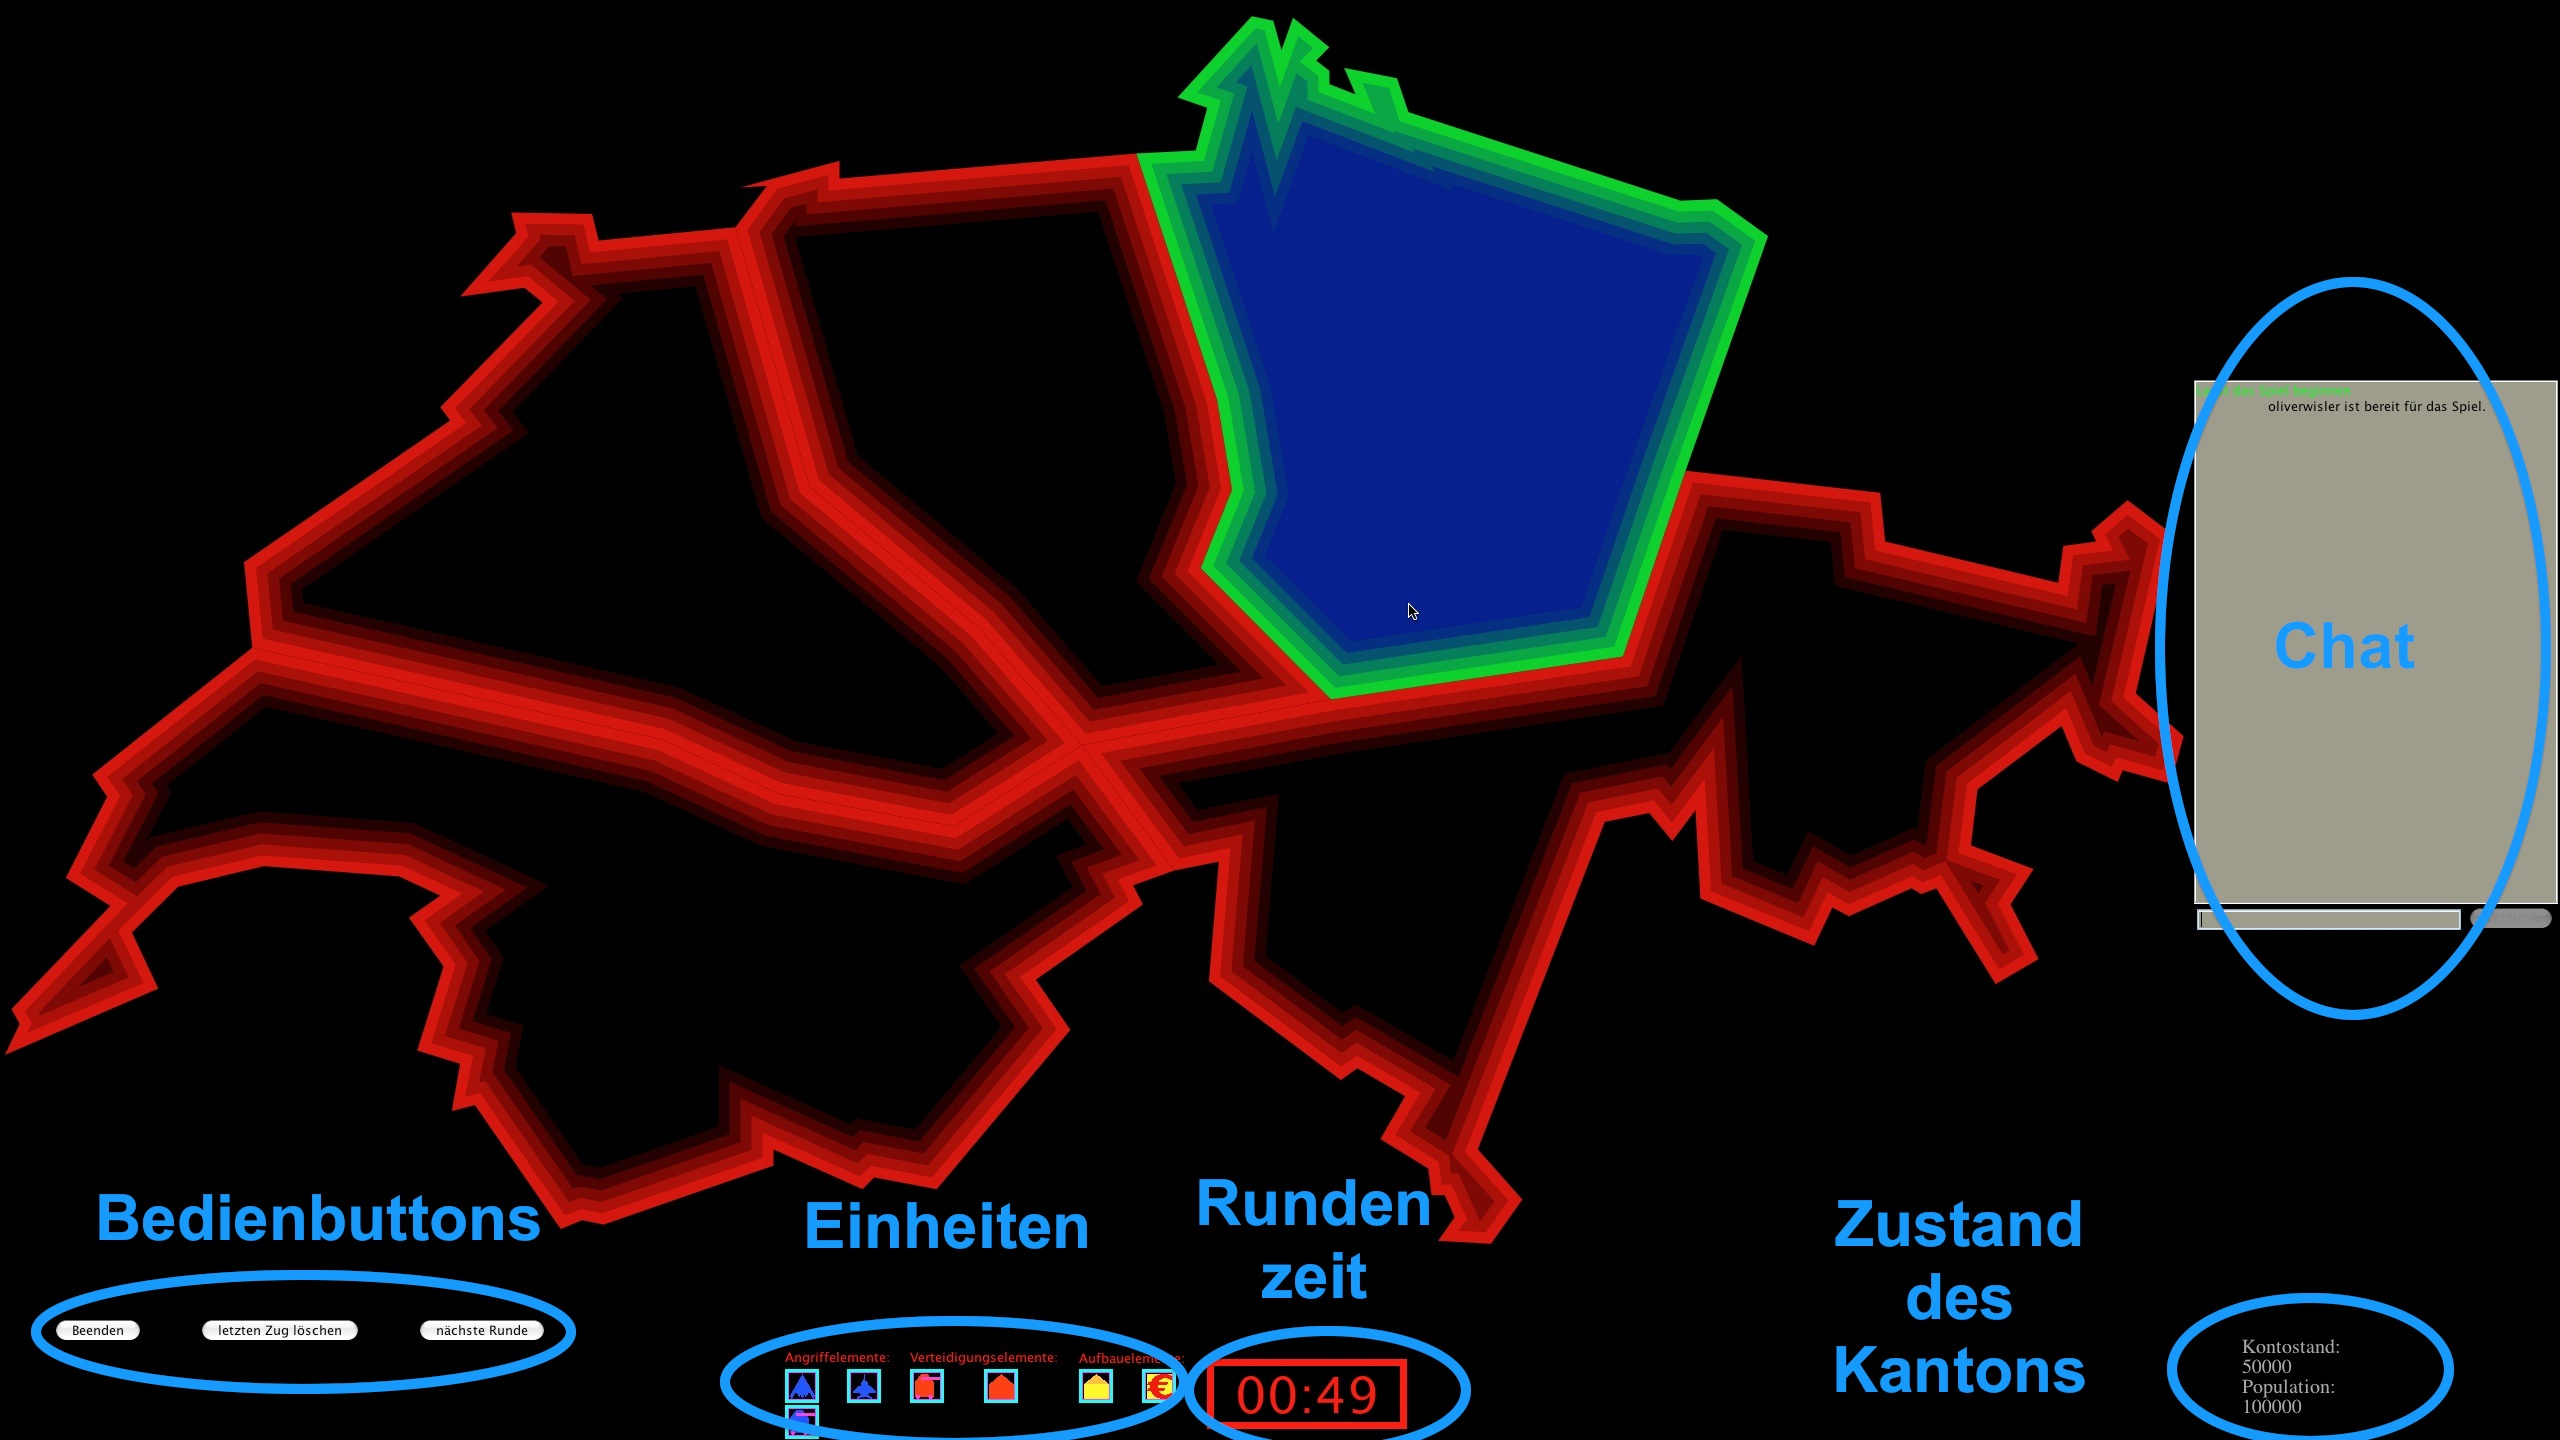
\includegraphics[scale=0.15]{spiel/spielfenster.jpg}
\caption{Spielfenster}
\end{figure}


Ziel des Spiels ist es die gegnerische Bevölkerung auszulöschen. Hat ein Spieler keine Bevölkerung mehr scheidet er aus dem Spiel aus.
Hierzu hat jeder Spieler zu Beginn des Spiels eine bestimmte Anzahl an Bevölkerung, sowie Geld zur verfügung.
Mit dem Geld hat man die Möglichkeit Gebäude (Banken und Reproduktionszentren), Abwehrelemente (Luft- und Landabwehr), sowie Angriffselemente (Bomber, Panzer und Jets) zu kaufen. Mit denen hat man die Möglichkeit sich zu schützen, wieder Aufzubauen oder Anzugreifen. Nähere Informationen findest du im Kapitel \ref{subsec:Einheit} Einheiten.

\newpage

\subsection{Spielfeld}
Das Feld mit dem blau-grauen Hintergrund ist dein Kanton. Deine Einheiten werden blau umrandet, während gegnerische Einheiten jeweils mit einer anderen Farbe gekennzeichnet werden.
\begin{figure}[h!]
\centering
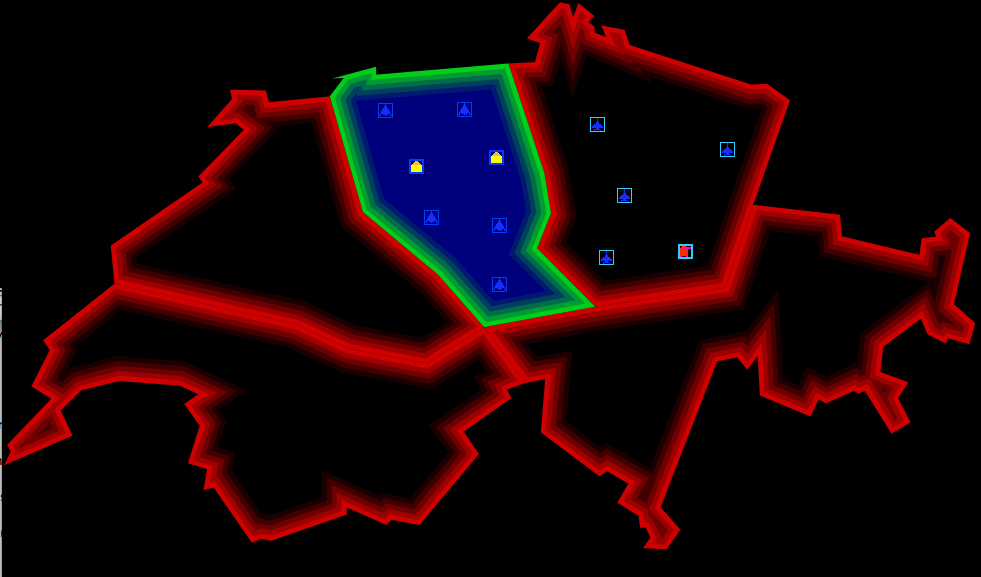
\includegraphics[scale=0.4]{spiel/map_with_units.png}
\caption{Spielfeld mit Einheiten}
\end{figure}
Wenn du deine Einheiten verschiebst, so wird dies mit einem gelben Pfeil markiert. Einheiten die sich seit der letzten Runde verschoben haben werden mit einem roten Pfeil angezeigt.

Das Spielfeld Besteht aus der Schweizerkarte, die in fünf Felder aufgeteilt ist. Das eigene Feld ist Grün umrandet und hat einen blauen Hintergrund. Die Felder der Gegner haben alle eine rote Umrandung auf schwarzem Hintergrund.

\begin{figure}[h]
\centering
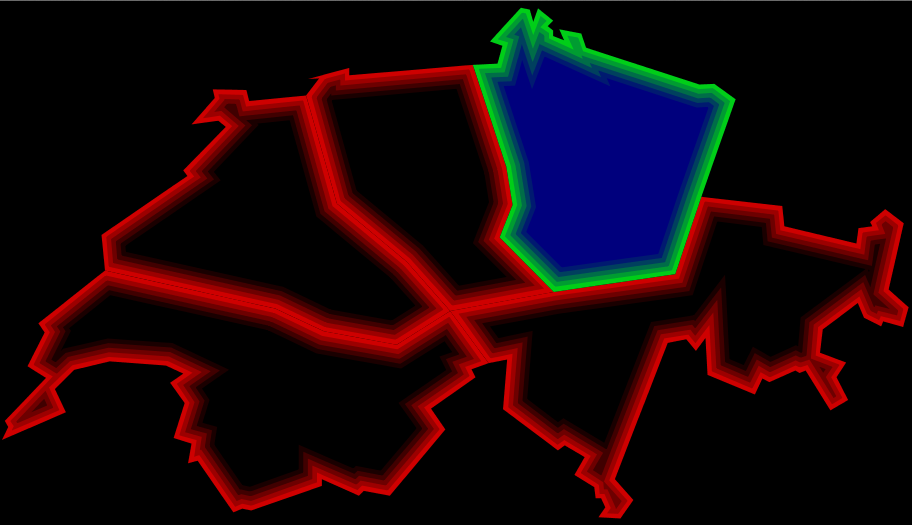
\includegraphics[scale=0.3]{spiel/spielfeld.png}
\caption{Spielfeld}
\end{figure}

%Das Fenster des Spiels besteht aus verschiedenen Elementen. eines ist das oben vorgestellte Spielfeld, ein anderes ist der Chat auf der rechten Seite(1), die Buttons um Objekte zu setzten(2),
%Buttons um ein Spiel zu beenden, den letzten Zug zu löschen oder um zu zeigen, dass man bereit ist um eine neue Runde zu Spielen(5), ein Timer(3), der die restliche Spielzeit in dieser Runde anzeigt, sowie die Information über das aktuelle Kontoinhaben und die Population(4).
%
%\begin{figure}[h]
%\centering
%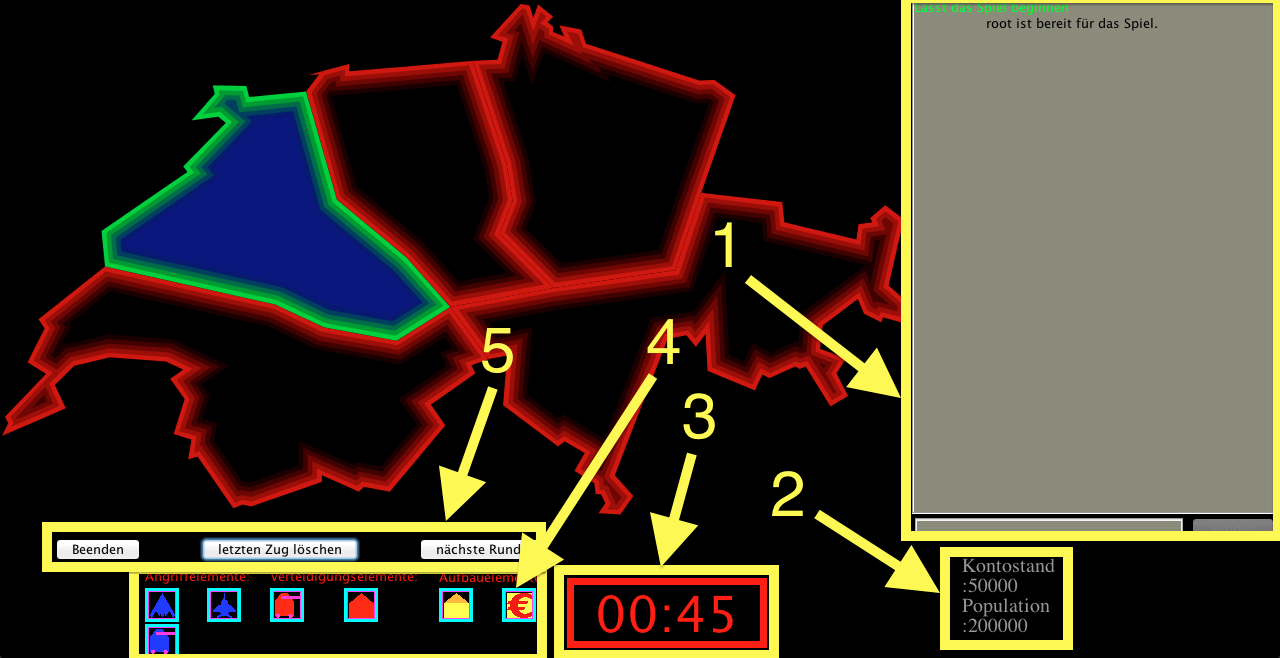
\includegraphics[scale=0.3]{spiel/spielfenster.png}
%\caption{Fenster in dem das Spiel stattfindet}
%\end{figure}

\newpage

\subsection{Einheiten} \label{subsec:Einheit}

Es gibt folgende Spielfiguren: 
\begin{itemize}
\item Bomber
\item Panzer
\item Jet
\item Flugabwehr
\item Landabwehr
\item Bank
\item  Reproduktionszentrum
\end{itemize}

\subsubsection{Bomber}

\begin{figure}[h]
\centering

\includegraphics[scale=1.8]{einheiten/Bomber.png}
\caption{Bomber}
\end{figure}

Der Bomber ist ein Angriffsobjekt.
Er wird auf den eigenen Kanton gesetzt. Um einen Zug zu tätigen muss er angewählt werden und seine Zieldestination kann gesetzt werden. Seine spezielle Eigenschaft ist, dass er als einziger nach jeder Runde direkt wieder zurück an seinen Startort fliegt.
Seine Ziele sind einerseits Gebäude aber auch die Bevölkerung eines Landes. Seine Reichweite sind 200'000 km.

\newpage

\subsubsection{Panzer}

\begin{figure}[h]
\centering
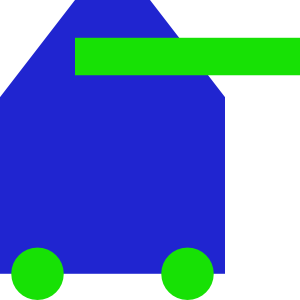
\includegraphics[scale=1.8]{einheiten/Panzer.png}
\caption{Panzer}
\end{figure}

Der Panzer ist ebenfalls ein Angriffselement.
Mit seinem Bewegungsradius von 30'000 km hat er die kleinste Reichweite pro Zug. Er greift alles, dass um ihn herum ist an, sei es Bevölkerung oder Gebäude. 


\subsubsection{Jet}

\begin{figure}[h]
\centering

\includegraphics[scale=1.8]{einheiten/Flugzeug.png}
\caption{Jet}
\end{figure}

Genau wie der Bomber und der Panzer ist der Jet ebenfalls ein Angriffselement.
Seine Aufgabe ist es, die eigenen Bomber zu eskortieren. Er kann lediglich andere Bomber und Flugabwehr angreifen. Mit einer Reichweite von 50'000 km pro Runde liegt er im Mittelwert.

\newpage

\subsubsection{Landabwehr}


\begin{figure}[h]
\centering

\includegraphics[scale=1.8]{einheiten/Landabwehr.png}
\caption{Landabwehr}
\end{figure}

Die Landabwehr ist ein Abwehrelement. Es kann wie alle Abwehrelemente nur in dem eigenen Kanton gebaut werden und danach nicht mehr verschoben werden. Seine Aufgabe ist es Gebäude und die Bevölkerung vor gegnerischen Panzern zu schützen.


\newpage

\subsubsection{Flugabwehr}

\begin{figure}[h]
\centering

\includegraphics[scale=18]{einheiten/Flugabwehr.png}
\caption{Flugabwehr}
\end{figure}

Die Flugabwehr ist das zweite Abwehrelement. Es kann Jet und Bomber Angreifen, die den eigenen Kanton versuchen anzugreifen.


\subsubsection{Bank}

\begin{figure}[h]
\centering

\includegraphics[scale=1.8]{einheiten/Bank.png}
\caption{Bank}
\end{figure}

Die Bank ist eines der Beiden Aufbauelemente. Die Bank wird in dem eigenen Kanton gebaut und sorgt für zusätzliches Geld in der Kommenden Runde. Jede Bank bringt dem Besitzer ein Plus von 1000 Geld pro Spielrunde.

\newpage

\subsubsection{Reproduktionszentrum}

\begin{figure}[h]
\centering

\includegraphics[scale=2]{einheiten/Repro.png}
\caption{Reproduktionszentrum}
\end{figure}

Mit dem Reproduktionszentrum kann die Bevölkerung vermehrt werden. Sie bringt pro Runde 100 neue Bevölkerung.

\newpage

\subsection{Einheiten platzieren}

Einheiten können folgendermassen plaziert werden. 

\begin{figure}[h]
\centering
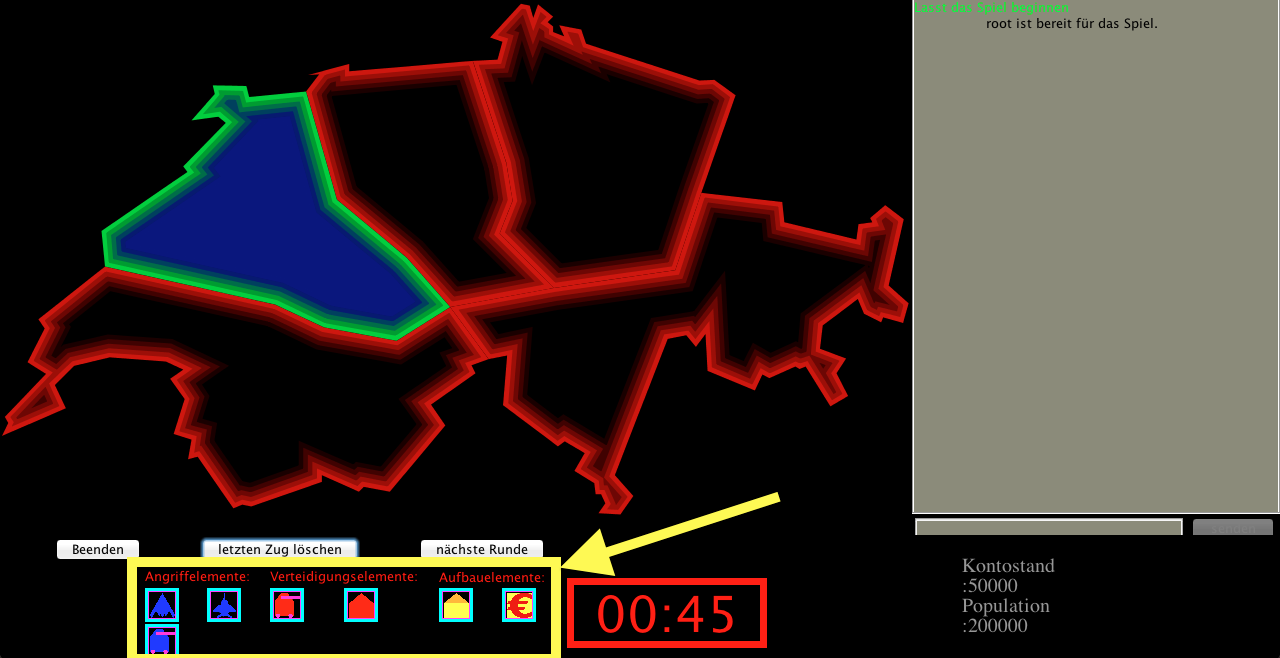
\includegraphics[scale=0.3]{spiel/Objekt_aussuchen.png}
\caption{Objekt wählen}
\end{figure}

Zuerst muss das gewünschte Objekt, dass gebildet werden soll durch Mausklick ausgesucht werden. Der Hintergrund des ausgesuchten Objektes unterscheidet sich farblich von den anderen.

\begin{figure}[h]
\centering
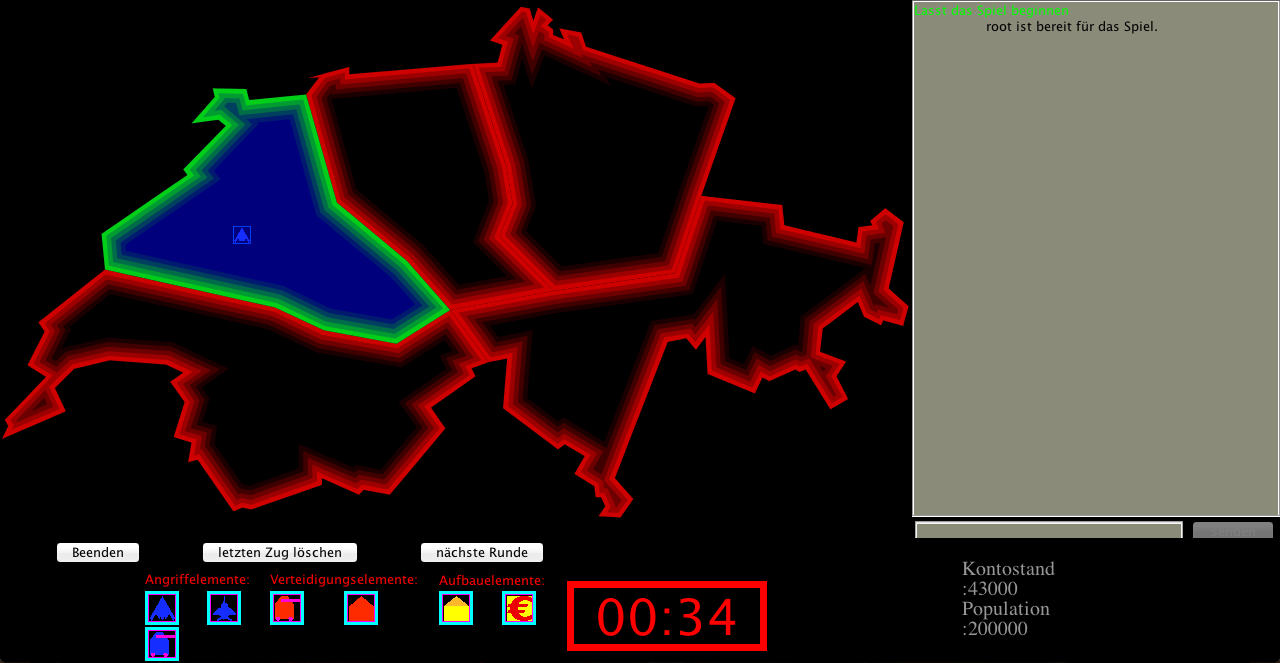
\includegraphics[scale=0.3]{spiel/Objekt_setzen.png}
\caption{Objekt auf Kanton setzten}
\end{figure}

Als nächstes muss das Objekt auf der Karte platziert werden. Dazu einfach per Mausklick auf den eigenen Kanton setzten. Ist der Zug ungültig, da man kein Geld mehr hat oder das Objekt an einen unzulässigen Platz gesetzt wird, so wird er nicht ausgeführt.

\newpage

\subsection{Einheiten verschieben}

\begin{figure}[h]
\centering
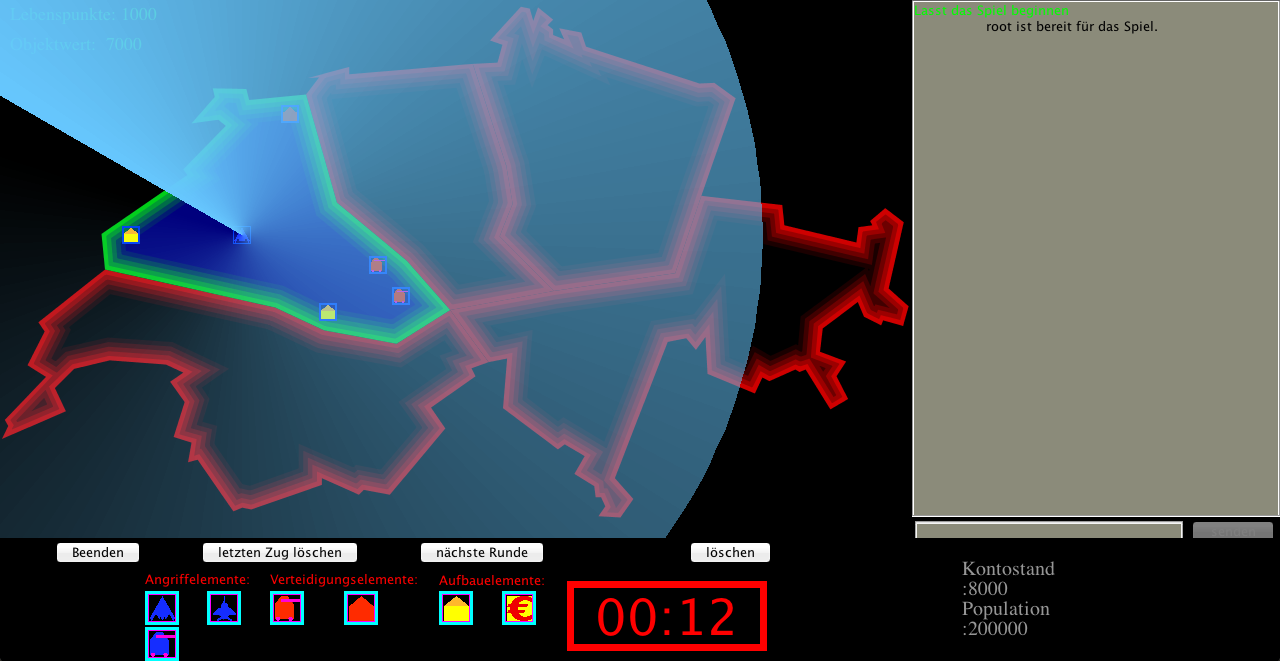
\includegraphics[scale=0.28]{spiel/Objekt_anwaehlen.png}
\caption{Objekt anw\"{a}hlen}
\end{figure}

Um ein Objekt zu verschieben, muss dieses zuerst angew\"{a}hlt werden. Daf\"{u}hr drückt man lediglich auf der Spielfläche auf das gewünschte Objekt. Danach erscheint ein blauer Radar, welcher den Radius darstellt, um welchen das Objekt verschoben werden kann. Zudem wird oben Links auf der Karte die aktuellen Lebenspunkte, sowie der Geldwert angezeigt. Zudem erscheint ein Löschknopf, mit dem das angewählte Objekt gelöscht werden kann.

Um den Bestimmungsort des Objektes zu wählen musst du per Maus innerhalb des Radius drücken. Danach wird ein Pfeil vom alten an den neuen Ort gezeichnet.
\begin{figure}[h]
\centering
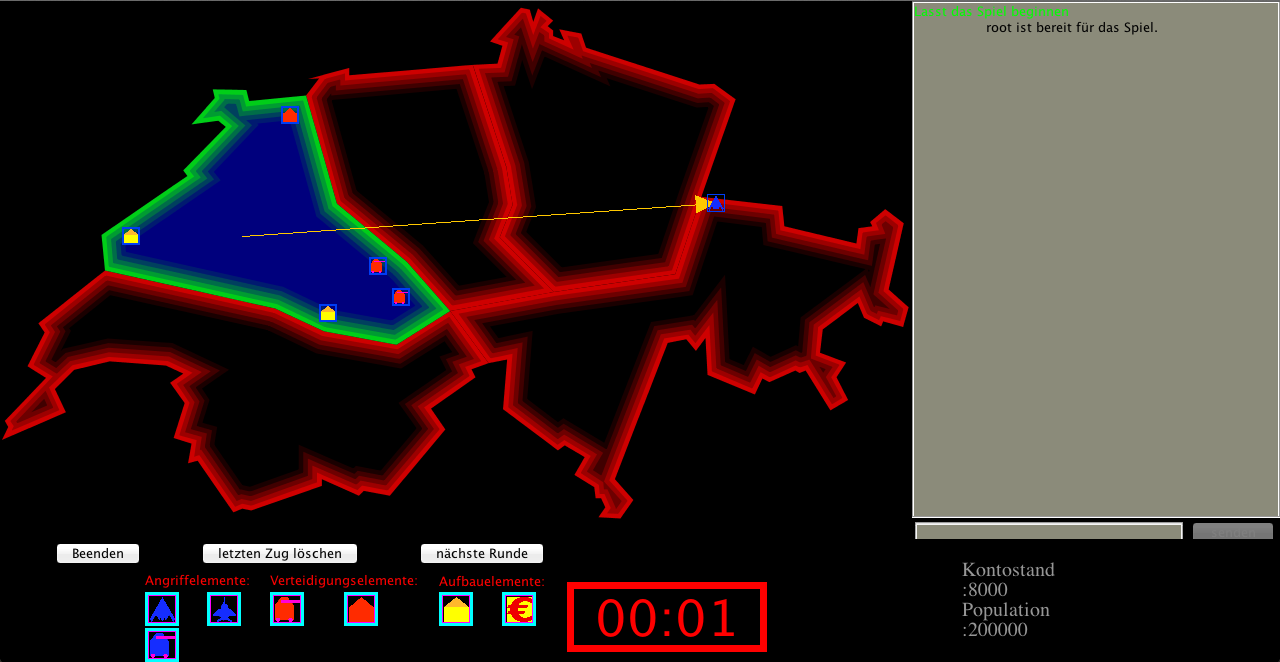
\includegraphics[scale=0.28]{spiel/Objekt_verschieben.png}
\caption{Objekt verschieben}
\end{figure}

Möchte man keinen Zug mit diesem Objekt vollziehen, so klickt man ausserhalb des Radars auf den Bildschirm und das Objekt wird abgewählt.

\newpage

\subsection{Nach der Erstellungs-Phase}

Ist die Erstellungsphase beendet, so ist nichts mehr anwählbar und du bekommst falls du noch versuchst weiter zu setzten eine Meldung.
Nach dieser Phase siehst du, was deine Gegner in der letzten Runde für Objekte erstellt hat, jeder Spieler hat eine andere Farbe, mit der seine Objekte umrandet sind. Zudem wird sich deine Population und Kontostand verändern, da die Aktionen ausgeführt werden.

\begin{figure}[h]
\centering
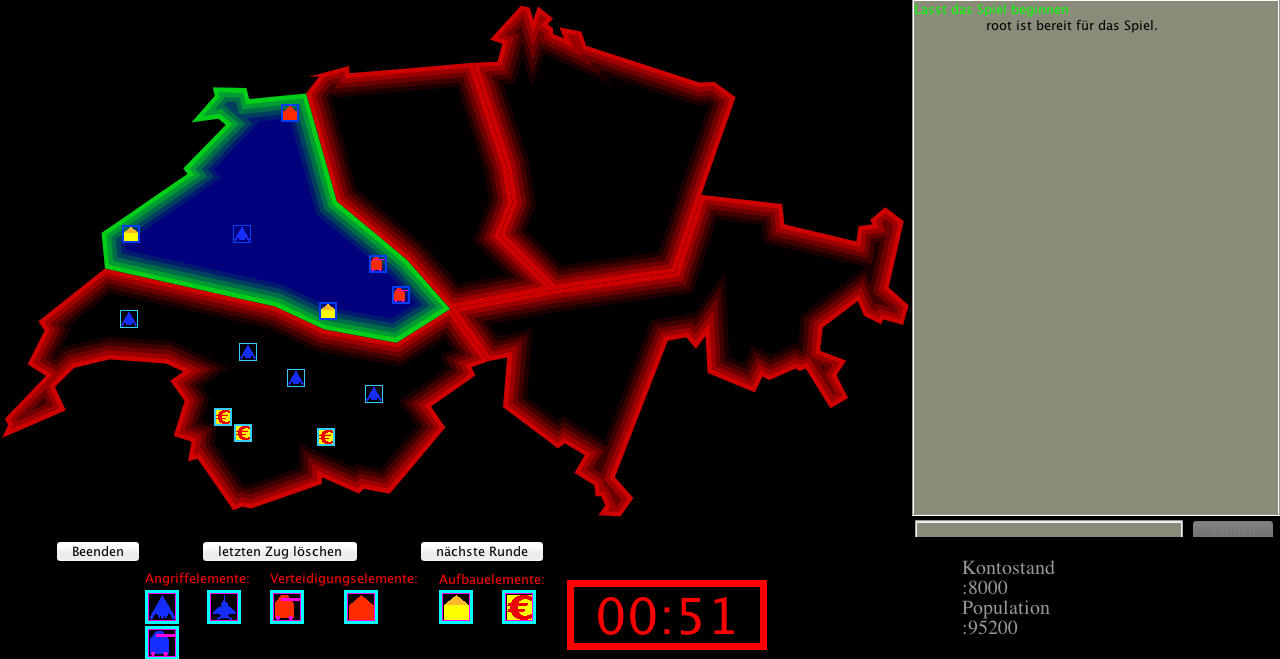
\includegraphics[scale=0.3]{spiel/Objekt_gegner.png}
\caption{Objekt aller Gegner}
\end{figure}

\newpage

\subsection{Gewinner und Verlierer}

Verlässt ein Spieler das Spiel oder hat er keine Population mehr, so verliert er dieses. Sind noch mehr als 1 Spieler in einem Spiel aktiv, so spielen diese weiter.
Dem Verlierer wird folgende Meldung angezeigt:

\begin{figure}[h]
\centering
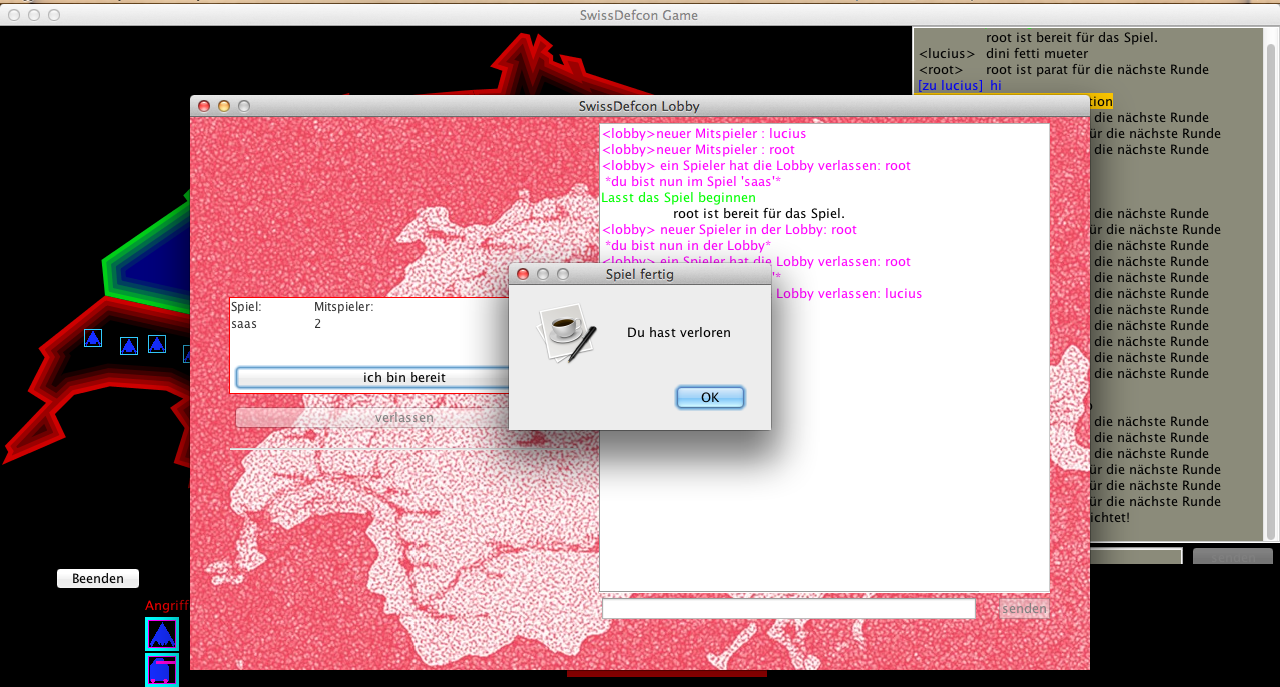
\includegraphics[scale=0.29]{spiel/verloren.png}
\caption{Ausgabe beim Verlierer}
\end{figure}

Die anderen Spieler spielen so lange weiter, bis nur noch ein Spieler übrig bleibt. Wer ausgeschieden ist, hat jedoch die Möglichkeit bei dem Spiel weiter zuzuschauen.
Dem Gewinner wird nach dem Spiel folgendes angezeigt:

\begin{figure}[h]
\centering
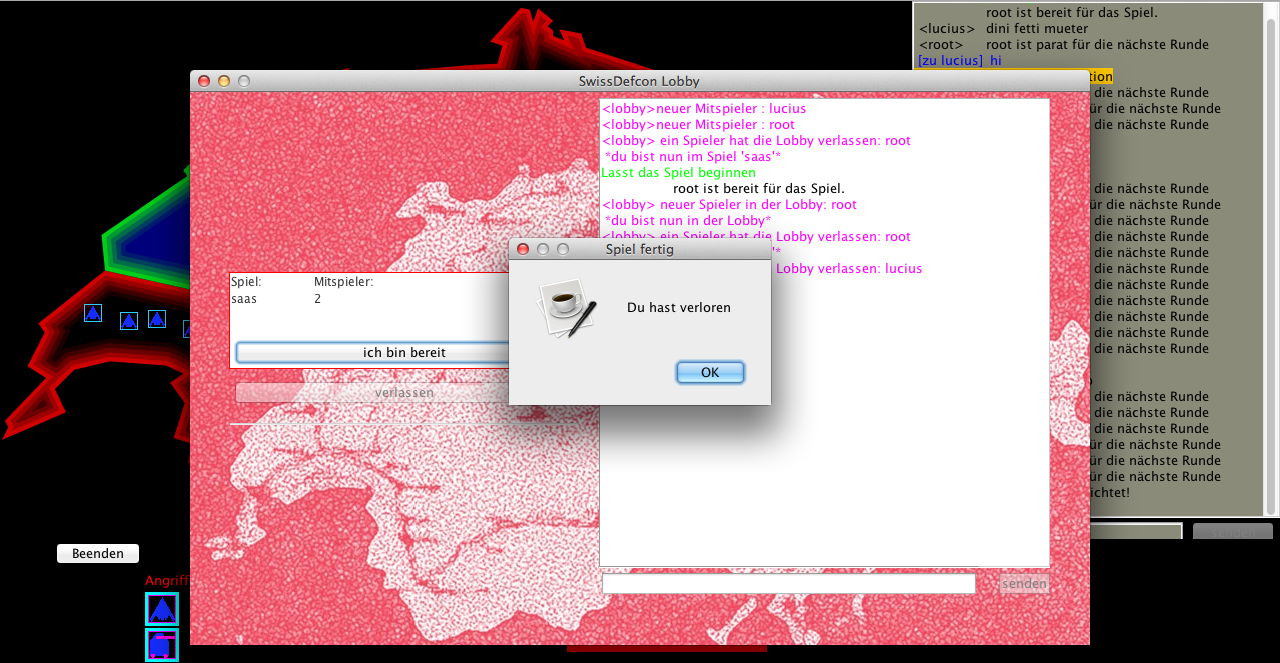
\includegraphics[scale=0.29]{spiel/gewonnen.png}
\caption{Ausgabe beim Gewinner}
\end{figure}

Wenn das Spiel zu Ende ist, oder ein Spieler das Spiel verlässt, gelangt er zurück in die Lobby, wo neue Spiele gestartet werden können.

\end{document}
